
%%%%%%%%%%%%%%
%            %
% Guidance   %
%            %
\chapter{\color{red}Guidance}
\label{cp:gd}

%\begin{highlight}
%    \begin{st}
%        General structure with just some dummy text.
%    \end{st} 
%\end{highlight}

%\lettrine{A}{a}


\section{\color{red}Vector Fields for Guidance}

The use of vector fields for guidance is widely discussed in the literature~\citep{lindemann2005smoothly,gonccalves2010vector,panagou2014motion,zhou2014vector,kapitanyuk2017guiding,de2017guidance}.

\begin{figure}[h]
  \centering
  
\definecolor{c2B2B2B}{RGB}{43,43,43}
\definecolor{cDEDEDE}{RGB}{222,222,222}
\definecolor{c989898}{RGB}{152,152,152}
\definecolor{cFFFFFF}{RGB}{255,255,255}
\definecolor{c4D4D4D}{RGB}{77,77,77}
\definecolor{c9B9B9B}{RGB}{155,155,155}


\def \globalscale {1.000000}
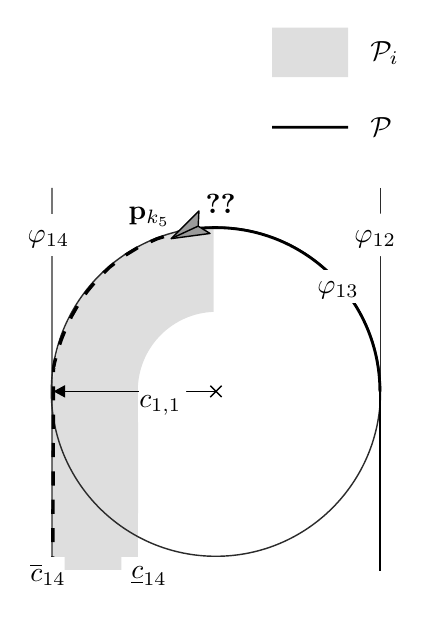
\begin{tikzpicture}[y=0.80pt, x=0.80pt, yscale=-1.2*\globalscale, xscale=1.2*\globalscale, inner sep=0pt, outer sep=0pt]



\path[draw=c2B2B2B,line join=round,line width=0.512pt] (137.9100,95.3391) -- (137.9100,239.5120);



  \path[fill=cFFFFFF,line join=round,line width=0.160pt] (144.6860,105.0630) -- (131.2360,105.0630) -- (131.2360,121.0330) -- (144.6960,121.0670) -- (144.6860,105.0630) -- cycle;



  \path[cm={{1.0,0.0,0.0,1.0,(128.0,118.0)}}] (0.0000,0.0000) node[above right] () {$\varphi_{12}$};



\path[fill=cDEDEDE,line join=round,line width=0.160pt] (14.4062,169.9360) -- (14.4311,169.9360) .. controls (15.3584,137.0320) and (42.0351,110.5710) .. (75.0243,109.9900) -- (75.0243,142.0480) .. controls (59.7109,142.6110) and (47.3600,154.7750) .. (46.5019,170.0120) -- (46.5148,182.6390) -- (46.5019,182.9250) -- (46.5019,183.2150) .. controls (46.5154,183.9430) and (46.6203,184.7000) .. (46.6001,185.4160) -- (46.6055,185.4230) -- (46.6055,187.1950) -- (46.5019,227.3090) -- (46.5019,234.5270) -- (46.4833,234.5270) -- (46.4830,234.6700) -- (46.4723,235.4800) -- (46.5303,239.1710) -- (14.2304,239.1780) .. controls (14.2304,237.5050) and (14.2092,240.8130) .. (14.1991,237.1110) -- (14.1991,235.5690) -- (14.1991,235.2560) -- (14.1991,234.8370) -- (14.1991,234.5320) -- (14.1991,171.8980) -- (14.4062,169.9360) -- cycle;



\path[draw=c2B2B2B,line join=round,line width=0.512pt] (75.8516,172.0930) ellipse (1.7421cm and 1.7421cm);



\path[draw=black,line join=round,line width=0.512pt] (78.0152,174.1270) -- (73.7395,169.8460);



\path[draw=black,line join=round,line width=0.512pt] (73.7417,174.1270) -- (78.0230,169.8460);



\path[draw=c2B2B2B,line join=round,line width=0.512pt] (14.1483,95.3578) -- (14.1477,239.5310);



\path[draw=black,line join=round,line width=0.512pt] (75.9234,172.0190) -- (14.0743,172.0190);



\path[fill=black,line join=round,line width=0.160pt] (19.0789,174.3350) -- (19.0727,169.6190) -- (14.7563,171.9820) -- (19.0789,174.3350) -- cycle;



  \path[fill=cFFFFFF,line join=round,line width=0.160pt,rounded corners=0.0000cm] (8.0901,105.0980) rectangle (20.5396,121.0676);



  \path[cm={{1.0,0.0,0.0,1.0,(5.0,118.0)}}] (0.0000,0.0000) node[above right] () {$\varphi_{14}$};



\path[draw=black,line join=round,line width=1.024pt] (67.5256,111.0380) .. controls (69.2504,110.2990) and (75.8630,110.3510) .. (75.8630,110.3510) .. controls (109.9540,110.3510) and (137.5900,137.9880) .. (137.5900,172.0790);



  \path[fill=cFFFFFF,line join=round,line width=0.160pt,rounded corners=0.0000cm] (115.2640,126.2090) rectangle (131.2335,138.6585);



  \path[cm={{1.0,0.0,0.0,1.0,(114.0,137.0)}}] (0.0000,0.0000) node[above right] () {$\varphi_{13}$};



  \path[fill=cFFFFFF,line join=round,line width=0.160pt] (52.6996,234.3410) -- (40.2501,234.3410) -- (40.2318,246.3700) -- (52.7105,246.3700) -- (52.6996,234.3410) -- cycle;



  \path[cm={{1.0,0.0,0.0,1.0,(44.0,245.0)}}] (0.0000,0.0000) node[above right] () {$\underline{c}_{14}$};



  \path[fill=cFFFFFF,line join=round,line width=0.160pt] (64.6687,169.3940) -- (46.9391,169.3930) -- (46.9391,181.8430) -- (64.6687,181.8430) -- (64.6687,169.3940) -- cycle;



  \path[cm={{1.0,0.0,0.0,1.0,(47.0,181.0)}}] (0.0000,0.0000) node[above right] () {$c_{1,1}$};



\path[fill=black,line join=round,line width=0.256pt] (13.8207,228.7410) -- (13.8435,223.4080) -- (15.1234,223.4140) -- (15.1007,228.7470) -- (13.8207,228.7410) -- cycle(13.8662,218.0750) -- (13.8890,212.7420) -- (15.1690,212.7470) -- (15.1462,218.0800) -- (13.8662,218.0750) -- cycle(13.9117,207.4080) -- (13.9345,202.0750) -- (15.2145,202.0800) -- (15.1917,207.4140) -- (13.9117,207.4080) -- cycle(13.9572,196.7420) -- (13.9800,191.4080) -- (15.2600,191.4140) -- (15.2372,196.7470) -- (13.9572,196.7420) -- cycle(14.0028,186.0750) -- (14.0255,180.7420) -- (15.3055,180.7470) -- (15.2828,186.0810) -- (14.0028,186.0750) -- cycle(14.0483,175.4090) -- (14.0711,170.0750) -- (15.3510,170.0810) -- (15.3283,175.4140) -- (14.0483,175.4090) -- cycle(14.0938,164.7420) -- (14.1004,163.1940) -- (14.1116,163.0700) -- (14.1481,162.9500) -- (14.2078,162.8390) -- (14.2888,162.7440) -- (14.3849,162.6630) -- (14.4954,162.6040) -- (14.6155,162.5680) -- (14.7404,162.5570) -- (14.1975,162.5580) -- (14.4982,161.0400) -- (14.8987,159.3600) -- (16.1499,159.6300) -- (15.7494,161.3100) -- (15.4579,162.7820) -- (14.7404,163.8370) -- (15.3804,163.2000) -- (15.3738,164.7470) -- (14.0938,164.7420) -- cycle(16.4171,154.1910) -- (17.1786,151.9470) -- (18.2993,149.1670) -- (19.5002,149.6100) -- (18.3795,152.3900) -- (17.6397,154.5700) -- (16.4171,154.1910) -- cycle(20.5366,144.2860) -- (20.9681,143.3850) -- (23.1393,139.5830) -- (24.2741,140.1750) -- (22.1029,143.9770) -- (21.7089,144.7990) -- (20.5366,144.2860) -- cycle(26.1128,135.1000) -- (26.8488,134.0250) -- (29.4547,130.8780) -- (30.4785,131.6470) -- (27.8725,134.7930) -- (27.1990,135.7770) -- (26.1128,135.1000) -- cycle(33.1525,126.9590) -- (35.2417,124.9010) -- (37.1822,123.3740) -- (38.0303,124.3330) -- (36.0897,125.8600) -- (34.0975,127.8220) -- (33.1525,126.9590) -- cycle(41.5104,120.1440) -- (46.0624,117.3650) -- (46.7947,118.4150) -- (42.2427,121.1940) -- (41.5104,120.1440) -- cycle(50.9592,115.0720) -- (53.4451,113.9480) -- (56.0106,113.1560) -- (56.4648,114.3530) -- (53.8993,115.1450) -- (51.5589,116.2030) -- (50.9592,115.0720) -- cycle(61.1063,111.5820) -- (61.2085,111.5500) -- (66.4314,110.6160) -- (66.7338,111.8590) -- (61.5109,112.7940) -- (61.5606,112.7790) -- (61.1063,111.5820) -- cycle(13.7752,239.4080) -- (13.7979,234.0750) -- (15.0779,234.0800) -- (15.0552,239.4130) -- (13.7752,239.4080) -- cycle;



\path[cm={{1.0,0.0,0.0,1.0,(43.0,110.0)}}] (0.0000,0.0000) node[above right] () {$\mathbf{p}_{k_5}$};

\path[cm={{1.0,0.0,0.0,1.0,(72.0,105.0)}}] (0.0000,0.0000) node[above right] () {\ref{sth:i}};

  \path[fill=cFFFFFF,line join=round,line width=0.160pt] (18.9147,234.3410) -- (6.4652,234.3410) -- (6.4316,246.4160) -- (18.9102,246.3850) -- (18.9147,234.3410) -- cycle;



  \path[cm={{1.0,0.0,0.0,1.0,(6.0,245.0)}}] (0.0000,0.0000) node[above right] () {$\overline{c}_{14}$};



\path[draw=black,fill=c9B9B9B,line join=round,line width=0.512pt] (58.9895,114.4960) -- (73.6370,112.5410) -- (69.1896,109.7900) -- (69.4587,104.0670) -- (58.9895,114.4960) -- cycle;



\path[draw=black,line join=round,line width=0.512pt] (59.2931,114.3470) -- (69.0932,109.8070);



\path[draw=black,line join=round,line width=1.024pt] (137.5900,239.4500) -- (137.5900,171.8800);



\path[fill=cDEDEDE,line join=round,even odd rule,line width=0.160pt] (97.0260,35.0828) -- (125.6100,35.0831) -- (125.6100,53.6677) -- (97.0260,53.6675) -- (97.0260,35.0828) -- cycle;



\path[cm={{1.0,0.0,0.0,1.0,(134.0,49.0)}}] (0.0000,0.0000) node[above right] () {$\mathcal{P}_i$};



\path[draw=black,line join=round,line width=1.024pt] (97.0260,72.5827) -- (125.6110,72.5829);



\path[cm={{1.0,0.0,0.0,1.0,(134.0,76.0)}}] (0.0000,0.0000) node[above right] () {$\mathcal{P}$};


\end{tikzpicture}


  \caption[Path parameter in the flight of an aerial robot]{A path parameter in the flight of an aerial robot can be used to alter the overall energy consumption}
  \label{fig:tee1}
\end{figure}
%\begin{figure}[h]
%  \centering
%  
\definecolor{c2B2B2B}{RGB}{43,43,43}
\definecolor{cDEDEDE}{RGB}{222,222,222}
\definecolor{c989898}{RGB}{152,152,152}
\definecolor{cFFFFFF}{RGB}{255,255,255}
\definecolor{c4D4D4D}{RGB}{77,77,77}
\definecolor{c9B9B9B}{RGB}{155,155,155}


\def \globalscale {1.000000}
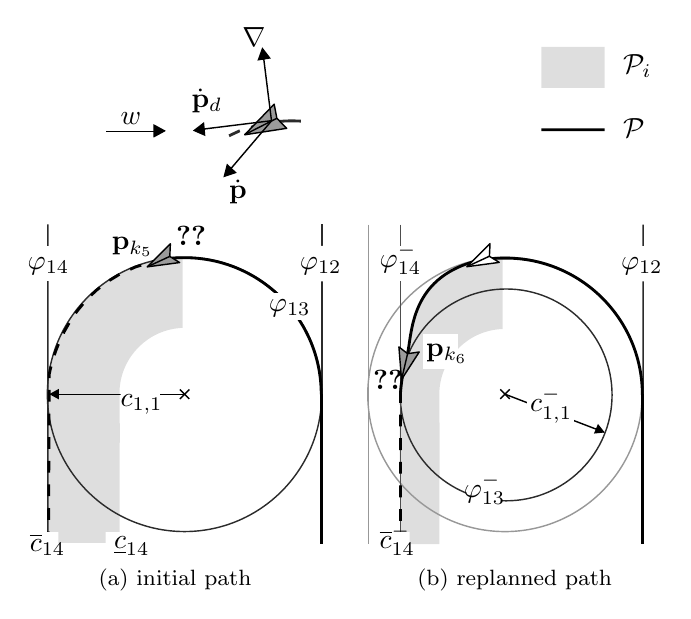
\begin{tikzpicture}[y=0.80pt, x=0.80pt, yscale=-\globalscale, xscale=\globalscale, inner sep=0pt, outer sep=0pt]
\path[fill=c2B2B2B,line join=round,line width=0.256pt] (101.0350,53.6179) -- (96.2027,55.8748) -- (95.7468,54.6788) -- (100.5790,52.4218) -- (101.0350,53.6179) -- cycle(111.1420,50.5445) -- (106.0290,52.0626) -- (105.7610,50.8111) -- (110.8730,49.2930) -- (111.1420,50.5445) -- cycle;



\path[draw=c2B2B2B,line join=round,line width=1.024pt] (128.3820,48.6757) .. controls (127.0480,48.5917) and (125.7060,48.5494) .. (124.3560,48.5494) .. controls (119.7720,48.5494) and (115.2670,49.0390) .. (110.8680,49.9835);



  \path[fill=cDEDEDE,line join=round,even odd rule,line width=0.160pt] (201.2220,113.9290) .. controls (207.0530,111.9750) and (213.0250,110.6150) .. (219.4860,110.5010) -- (219.4860,142.5600) .. controls (204.1730,143.1220) and (191.8220,155.2870) .. (190.9640,170.5230) -- (190.9770,183.1500) -- (190.9640,183.4360) -- (190.9640,183.7260) .. controls (190.9770,184.4540) and (191.0820,185.2110) .. (191.0620,185.9270) -- (191.0670,185.9340) -- (191.0670,187.7060) -- (190.9640,227.8200) -- (190.9640,235.0380) -- (190.9450,235.0380) -- (190.9450,235.1810) -- (190.9340,235.9910) -- (190.9920,239.6820) -- (173.2000,239.6860) .. controls (173.4790,219.6570) and (172.4790,191.1610) .. (173.3370,172.5260) .. controls (173.7560,163.4250) and (175.7760,156.4540) .. (176.3670,154.3980) .. controls (178.5870,146.6790) and (177.0030,123.9390) .. (200.7770,114.0980) -- (201.2220,113.9290) -- cycle;



  \path[draw=c989898,line join=round,line width=0.512pt] (220.5790,172.1070) ellipse (1.7421cm and 1.7421cm);



  \path[draw=black,line join=round,line width=0.512pt] (222.7480,174.1440) -- (218.4670,169.8620);



  \path[draw=c2B2B2B,line join=round,line width=0.512pt] (283.0110,95.4499) -- (283.0100,239.6230);



  \path[draw=black,line join=round,line width=1.024pt] (212.5660,111.2220) .. controls (214.2910,110.4830) and (220.9040,110.5350) .. (220.9040,110.5350) .. controls (254.9950,110.5350) and (282.6310,138.1720) .. (282.6310,172.2630);



  \path[draw=black,line join=round,line width=0.512pt] (218.4680,174.1410) -- (222.7490,169.8600);



    \path[fill=cFFFFFF,line join=round,line width=0.160pt] (289.4020,105.0980) -- (276.9530,105.0980) -- (276.9530,121.0670) -- (289.4080,121.0670) -- (289.4020,105.0980) -- cycle;



    \path[cm={{1.0,0.0,0.0,1.0,(273.0,118.0)}}] (0.0000,0.0000) node[above right] () {$\varphi_{12}$};



  \path[draw=black,line join=round,line width=1.024pt] (282.6300,239.6340) -- (282.6300,172.0640);



  \path[draw=c2B2B2B,line join=round,line width=0.512pt] (221.1170,172.3260) ellipse (1.3451cm and 1.3451cm);



  \path[draw=c4D4D4D,line join=round,line width=0.512pt] (173.4260,95.3725) -- (173.4260,239.5460);



  \path[draw=black,line join=round,line width=0.512pt] (265.2780,189.1390) -- (220.7780,172.0720);



  \path[draw=black,line join=round,line width=1.024pt] (212.0450,110.8620) .. controls (176.5020,117.4390) and (178.8960,145.6300) .. (176.3720,154.4050) .. controls (173.7630,163.4760) and (173.3650,171.9460) .. (173.3650,171.9460) -- (173.3790,172.2110) -- (173.4210,172.6590);



  \path[draw=black,fill=c9B9B9B,line join=round,line width=0.512pt] (173.8510,165.3770) -- (181.8430,152.9480) -- (176.6230,153.7110) -- (172.6800,150.6460) -- (173.8510,165.3770) -- cycle;



  \path[fill=black,line join=round,line width=0.256pt] (172.7330,229.2390) -- (172.7330,223.9060) -- (174.0130,223.9060) -- (174.0130,229.2390) -- (172.7330,229.2390) -- cycle(172.7330,218.5730) -- (172.7330,213.2390) -- (174.0130,213.2390) -- (174.0130,218.5730) -- (172.7330,218.5730) -- cycle(172.7330,207.9060) -- (172.7330,202.5730) -- (174.0130,202.5730) -- (174.0130,207.9060) -- (172.7330,207.9060) -- cycle(172.7330,197.2390) -- (172.7330,191.9060) -- (174.0130,191.9060) -- (174.0130,197.2390) -- (172.7330,197.2390) -- cycle(172.7330,186.5730) -- (172.7330,181.2390) -- (174.0130,181.2390) -- (174.0130,186.5730) -- (172.7330,186.5730) -- cycle(172.7330,175.9060) -- (172.7330,172.3360) -- (174.0130,172.3360) -- (174.0130,175.9060) -- (172.7330,175.9060) -- cycle(172.7330,239.9060) -- (172.7330,234.5730) -- (174.0130,234.5730) -- (174.0130,239.9060) -- (172.7330,239.9060) -- cycle;



    \path[fill=cFFFFFF,line join=round,line width=0.160pt,rounded corners=0.0000cm] (167.3680,105.0980) rectangle (179.8176,121.0676);



    \path[cm={{1.0,0.0,0.0,1.0,(164.0,118.0)}}] (0.0000,0.0000) node[above right] () {$\varphi_{14}^-$};



    \path[fill=cFFFFFF,line join=round,line width=0.160pt] (177.5750,234.3400) -- (165.1260,234.3400) -- (165.0920,246.4150) -- (177.5710,246.3840) -- (177.5750,234.3400) -- cycle;



    \path[cm={{1.0,0.0,0.0,1.0,(164.0,245.0)}}] (0.0000,0.0000) node[above right] () {$\overline{c}_{14}^-$};



    \path[fill=cFFFFFF,line join=round,line width=0.160pt,rounded corners=0.0000cm] (230.3230,173.2320) rectangle (251.5725,189.2016);



    \path[cm={{1.0,0.0,0.0,1.0,(232.0,185.0)}}] (0.0000,0.0000) node[above right] () {$c_{1,1}^-$};



  \path[draw=black,fill=cFFFFFF,line join=round,line width=0.512pt] (203.3560,114.4210) -- (218.0050,112.4770) -- (213.5600,109.7230) -- (213.8340,104.0000) -- (203.3560,114.4210) -- cycle;



    \path[fill=cFFFFFF,line join=round,line width=0.160pt] (199.4770,144.8830) -- (183.5080,144.8830) -- (183.5080,160.8530) -- (199.4770,160.8530) -- (199.4770,144.8830) -- cycle;



    \path[cm={{1.0,0.0,0.0,1.0,(185.0,158.0)}}] (0.0000,0.0000) node[above right] () {$\mathbf{p}_{k_6}$};

    \path[cm={{1.0,0.0,0.0,1.0,(161.0,170.0)}}] (0.0000,0.0000) node[above right] () {\ref{sth:iii}};

    \path[fill=cFFFFFF,line join=round,line width=0.160pt,rounded corners=0.0000cm] (192.4050,96.8819) rectangle (204.8546,109.3314);


  \path[draw=black,line join=round,line width=0.512pt] (203.7170,114.2570) -- (213.5160,109.7120);



  \path[draw=black,line join=round,line width=0.512pt] (174.0250,164.7330) -- (176.5840,153.7760);



    \path[fill=cFFFFFF,line join=round,line width=0.160pt] (219.2260,208.5700) -- (203.2560,208.5700) -- (203.2560,224.5400) -- (219.2260,224.5390) -- (219.2260,208.5700) -- cycle;



    \path[cm={{1.0,0.0,0.0,1.0,(202.0,222.0)}}] (0.0000,0.0000) node[above right] () {$\varphi_{13}^-$};



  \path[draw=c989898,line join=round,line width=0.512pt] (158.8570,95.3893) -- (158.8570,239.5620);



  \path[cm={{1.0,0.0,0.0,1.0,(181.0,261.0)}}] (0.0000,0.0000) node[above right] () {\footnotesize (b) replanned path};



  \path[fill=black,line join=round,line width=0.160pt] (262.5930,185.4440) -- (260.7610,189.7900) -- (265.6570,189.2950) -- (262.5930,185.4440) -- cycle;



\path[draw=c2B2B2B,line join=round,line width=0.512pt] (137.9100,95.3391) -- (137.9100,239.5120);



  \path[fill=cFFFFFF,line join=round,line width=0.160pt] (144.6860,105.0630) -- (131.2360,105.0630) -- (131.2360,121.0330) -- (144.6960,121.0670) -- (144.6860,105.0630) -- cycle;



  \path[cm={{1.0,0.0,0.0,1.0,(128.0,118.0)}}] (0.0000,0.0000) node[above right] () {$\varphi_{12}$};



\path[fill=cDEDEDE,line join=round,line width=0.160pt] (14.4062,169.9360) -- (14.4311,169.9360) .. controls (15.3584,137.0320) and (42.0351,110.5710) .. (75.0243,109.9900) -- (75.0243,142.0480) .. controls (59.7109,142.6110) and (47.3600,154.7750) .. (46.5019,170.0120) -- (46.5148,182.6390) -- (46.5019,182.9250) -- (46.5019,183.2150) .. controls (46.5154,183.9430) and (46.6203,184.7000) .. (46.6001,185.4160) -- (46.6055,185.4230) -- (46.6055,187.1950) -- (46.5019,227.3090) -- (46.5019,234.5270) -- (46.4833,234.5270) -- (46.4830,234.6700) -- (46.4723,235.4800) -- (46.5303,239.1710) -- (14.2304,239.1780) .. controls (14.2304,237.5050) and (14.2092,240.8130) .. (14.1991,237.1110) -- (14.1991,235.5690) -- (14.1991,235.2560) -- (14.1991,234.8370) -- (14.1991,234.5320) -- (14.1991,171.8980) -- (14.4062,169.9360) -- cycle;



\path[draw=c2B2B2B,line join=round,line width=0.512pt] (75.8516,172.0930) ellipse (1.7421cm and 1.7421cm);



\path[draw=black,line join=round,line width=0.512pt] (78.0152,174.1270) -- (73.7395,169.8460);



\path[draw=black,line join=round,line width=0.512pt] (73.7417,174.1270) -- (78.0230,169.8460);



\path[draw=c2B2B2B,line join=round,line width=0.512pt] (14.1483,95.3578) -- (14.1477,239.5310);



\path[draw=black,line join=round,line width=0.512pt] (75.9234,172.0190) -- (14.0743,172.0190);



\path[fill=black,line join=round,line width=0.160pt] (19.0789,174.3350) -- (19.0727,169.6190) -- (14.7563,171.9820) -- (19.0789,174.3350) -- cycle;



  \path[fill=cFFFFFF,line join=round,line width=0.160pt,rounded corners=0.0000cm] (8.0901,105.0980) rectangle (20.5396,121.0676);



  \path[cm={{1.0,0.0,0.0,1.0,(5.0,118.0)}}] (0.0000,0.0000) node[above right] () {$\varphi_{14}$};



\path[draw=black,line join=round,line width=1.024pt] (67.5256,111.0380) .. controls (69.2504,110.2990) and (75.8630,110.3510) .. (75.8630,110.3510) .. controls (109.9540,110.3510) and (137.5900,137.9880) .. (137.5900,172.0790);



  \path[fill=cFFFFFF,line join=round,line width=0.160pt,rounded corners=0.0000cm] (115.2640,126.2090) rectangle (131.2335,138.6585);



  \path[cm={{1.0,0.0,0.0,1.0,(114.0,137.0)}}] (0.0000,0.0000) node[above right] () {$\varphi_{13}$};



  \path[fill=cFFFFFF,line join=round,line width=0.160pt] (52.6996,234.3410) -- (40.2501,234.3410) -- (40.2318,246.3700) -- (52.7105,246.3700) -- (52.6996,234.3410) -- cycle;



  \path[cm={{1.0,0.0,0.0,1.0,(44.0,245.0)}}] (0.0000,0.0000) node[above right] () {$\underline{c}_{14}$};



  \path[fill=cFFFFFF,line join=round,line width=0.160pt] (64.6687,169.3940) -- (46.9391,169.3930) -- (46.9391,181.8430) -- (64.6687,181.8430) -- (64.6687,169.3940) -- cycle;



  \path[cm={{1.0,0.0,0.0,1.0,(47.0,181.0)}}] (0.0000,0.0000) node[above right] () {$c_{1,1}$};



\path[fill=black,line join=round,line width=0.256pt] (13.8207,228.7410) -- (13.8435,223.4080) -- (15.1234,223.4140) -- (15.1007,228.7470) -- (13.8207,228.7410) -- cycle(13.8662,218.0750) -- (13.8890,212.7420) -- (15.1690,212.7470) -- (15.1462,218.0800) -- (13.8662,218.0750) -- cycle(13.9117,207.4080) -- (13.9345,202.0750) -- (15.2145,202.0800) -- (15.1917,207.4140) -- (13.9117,207.4080) -- cycle(13.9572,196.7420) -- (13.9800,191.4080) -- (15.2600,191.4140) -- (15.2372,196.7470) -- (13.9572,196.7420) -- cycle(14.0028,186.0750) -- (14.0255,180.7420) -- (15.3055,180.7470) -- (15.2828,186.0810) -- (14.0028,186.0750) -- cycle(14.0483,175.4090) -- (14.0711,170.0750) -- (15.3510,170.0810) -- (15.3283,175.4140) -- (14.0483,175.4090) -- cycle(14.0938,164.7420) -- (14.1004,163.1940) -- (14.1116,163.0700) -- (14.1481,162.9500) -- (14.2078,162.8390) -- (14.2888,162.7440) -- (14.3849,162.6630) -- (14.4954,162.6040) -- (14.6155,162.5680) -- (14.7404,162.5570) -- (14.1975,162.5580) -- (14.4982,161.0400) -- (14.8987,159.3600) -- (16.1499,159.6300) -- (15.7494,161.3100) -- (15.4579,162.7820) -- (14.7404,163.8370) -- (15.3804,163.2000) -- (15.3738,164.7470) -- (14.0938,164.7420) -- cycle(16.4171,154.1910) -- (17.1786,151.9470) -- (18.2993,149.1670) -- (19.5002,149.6100) -- (18.3795,152.3900) -- (17.6397,154.5700) -- (16.4171,154.1910) -- cycle(20.5366,144.2860) -- (20.9681,143.3850) -- (23.1393,139.5830) -- (24.2741,140.1750) -- (22.1029,143.9770) -- (21.7089,144.7990) -- (20.5366,144.2860) -- cycle(26.1128,135.1000) -- (26.8488,134.0250) -- (29.4547,130.8780) -- (30.4785,131.6470) -- (27.8725,134.7930) -- (27.1990,135.7770) -- (26.1128,135.1000) -- cycle(33.1525,126.9590) -- (35.2417,124.9010) -- (37.1822,123.3740) -- (38.0303,124.3330) -- (36.0897,125.8600) -- (34.0975,127.8220) -- (33.1525,126.9590) -- cycle(41.5104,120.1440) -- (46.0624,117.3650) -- (46.7947,118.4150) -- (42.2427,121.1940) -- (41.5104,120.1440) -- cycle(50.9592,115.0720) -- (53.4451,113.9480) -- (56.0106,113.1560) -- (56.4648,114.3530) -- (53.8993,115.1450) -- (51.5589,116.2030) -- (50.9592,115.0720) -- cycle(61.1063,111.5820) -- (61.2085,111.5500) -- (66.4314,110.6160) -- (66.7338,111.8590) -- (61.5109,112.7940) -- (61.5606,112.7790) -- (61.1063,111.5820) -- cycle(13.7752,239.4080) -- (13.7979,234.0750) -- (15.0779,234.0800) -- (15.0552,239.4130) -- (13.7752,239.4080) -- cycle;



\path[cm={{1.0,0.0,0.0,1.0,(43.0,110.0)}}] (0.0000,0.0000) node[above right] () {$\mathbf{p}_{k_5}$};

\path[cm={{1.0,0.0,0.0,1.0,(72.0,105.0)}}] (0.0000,0.0000) node[above right] () {\ref{sth:i}};

  \path[fill=cFFFFFF,line join=round,line width=0.160pt] (18.9147,234.3410) -- (6.4652,234.3410) -- (6.4316,246.4160) -- (18.9102,246.3850) -- (18.9147,234.3410) -- cycle;



  \path[cm={{1.0,0.0,0.0,1.0,(6.0,245.0)}}] (0.0000,0.0000) node[above right] () {$\overline{c}_{14}$};



\path[draw=black,fill=c9B9B9B,line join=round,line width=0.512pt] (58.9895,114.4960) -- (73.6370,112.5410) -- (69.1896,109.7900) -- (69.4587,104.0670) -- (58.9895,114.4960) -- cycle;



\path[draw=black,line join=round,line width=0.512pt] (59.2931,114.3470) -- (69.0932,109.8070);



\path[cm={{1.0,0.0,0.0,1.0,(37.0,261.0)}}] (0.0000,0.0000) node[above right] () {\footnotesize (a) initial path};



\path[draw=black,line join=round,line width=1.024pt] (137.5900,239.4500) -- (137.5900,171.8800);



\path[fill=cDEDEDE,line join=round,even odd rule,line width=0.160pt] (237.0260,15.0828) -- (265.6100,15.0831) -- (265.6100,33.6677) -- (237.0260,33.6675) -- (237.0260,15.0828) -- cycle;



\path[cm={{1.0,0.0,0.0,1.0,(274.0,29.0)}}] (0.0000,0.0000) node[above right] () {$\mathcal{P}_i$};



\path[draw=black,line join=round,line width=1.024pt] (237.0260,52.5827) -- (265.6110,52.5829);



\path[cm={{1.0,0.0,0.0,1.0,(274.0,56.0)}}] (0.0000,0.0000) node[above right] () {$\mathcal{P}$};



\path[draw=black,fill=c9B9B9B,line join=round,line width=0.512pt] (103.0020,54.8369) -- (121.9910,51.9150) -- (117.5520,47.3939) -- (116.3400,41.0080) -- (103.0020,54.8369) -- cycle;



\path[draw=black,line join=round,line width=0.512pt] (115.1520,48.6445) -- (111.3670,18.4898);



\path[draw=black,line join=round,line width=0.512pt] (115.2340,48.4465) -- (94.3696,72.9709);



\path[cm={{1.0,0.0,0.0,1.0,(102.0,15.0)}}] (0.0000,0.0000) node[above right] () {$\nabla\varPhi$};



\path[cm={{1.0,0.0,0.0,1.0,(96.0,86.0)}}] (0.0000,0.0000) node[above right] () {$\dot{\mathbf{p}}$};



\path[cm={{1.0,0.0,0.0,1.0,(79.0,45.0)}}] (0.0000,0.0000) node[above right] () {$\dot{\mathbf{p}}_d$};



\path[draw=black,line join=round,line width=0.512pt] (117.5520,47.3796) -- (103.1340,54.7265);



\path[fill=black,line join=round,line width=0.160pt] (99.4724,72.0401) -- (94.9925,67.8546) -- (93.3980,74.0506) -- (99.4724,72.0401) -- cycle;



\path[fill=black,line join=round,line width=0.160pt] (108.7830,21.3255) -- (114.8390,20.3742) -- (110.9400,15.3018) -- (108.7830,21.3255) -- cycle;



\path[fill=black,line join=round,line width=0.160pt] (79.6380,52.9767) -- (85.2585,55.4260) -- (84.6922,49.0532) -- (79.6380,52.9767) -- cycle;



\path[draw=black,line join=round,line width=0.512pt] (82.5181,52.4879) -- (114.8620,48.5042);



\path[draw=black,line join=round,line width=0.512pt] (40.3847,53.3572) -- (62.7169,53.3572);



\path[cm={{1.0,0.0,0.0,1.0,(47.0,50.0)}}] (0.0000,0.0000) node[above right] () {$w$};



\path[fill=black,line join=round,line width=0.160pt] (61.8249,50.0137) -- (61.8330,56.1447) -- (67.4450,53.0723) -- (61.8249,50.0137) -- cycle;




\end{tikzpicture}


%  \caption[Alteration of the path parameter]{The alteration of the path parameter $c_{1,1}$, the radius of the circle.}
%  \label{fig:tee2}
%\end{figure}

The set
\begin{equation}\label{eq:area}
  \mathcal{P}_i:=\{\mathbf{p}(t)\mid\varphi_i(\mathbf{p}(t),c_{i}^\rho),c_i^\rho\in\mathcal{U}_i\},
\end{equation}
delimits the area where the $i$th path $\varphi_i$ is free to evolve using the path parameters $c_i^\rho$ (the gray area in \fref{fig:tee1}{Figure}). $\varphi_i$ is a function of the two coordinates and the path parameters, and is equal to zero when a point $\mathbf{p}(t)$ is on the path. Physically, this means the aerial robot is flying exactly over the nominal trajectory. 

\begin{figure}[h]
  \centering
  
\definecolor{c2B2B2B}{RGB}{43,43,43}
\definecolor{cDEDEDE}{RGB}{222,222,222}
\definecolor{c989898}{RGB}{152,152,152}
\definecolor{cFFFFFF}{RGB}{255,255,255}
\definecolor{c4D4D4D}{RGB}{77,77,77}
\definecolor{c9B9B9B}{RGB}{155,155,155}


\def \globalscale {1.000000}
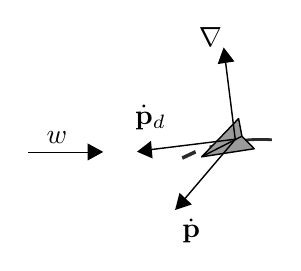
\begin{tikzpicture}[y=0.80pt, x=0.80pt, yscale=-1.25*\globalscale, xscale=1.25*\globalscale, inner sep=0pt, outer sep=0pt]
\path[fill=c2B2B2B,line join=round,line width=0.256pt] (101.0350,53.6179) -- (96.2027,55.8748) -- (95.7468,54.6788) -- (100.5790,52.4218) -- (101.0350,53.6179) -- cycle(111.1420,50.5445) -- (106.0290,52.0626) -- (105.7610,50.8111) -- (110.8730,49.2930) -- (111.1420,50.5445) -- cycle;



\path[draw=c2B2B2B,line join=round,line width=1.024pt] (128.3820,48.6757) .. controls (127.0480,48.5917) and (125.7060,48.5494) .. (124.3560,48.5494) .. controls (119.7720,48.5494) and (115.2670,49.0390) .. (110.8680,49.9835);





\path[draw=black,fill=c9B9B9B,line join=round,line width=0.512pt] (103.0020,54.8369) -- (121.9910,51.9150) -- (117.5520,47.3939) -- (116.3400,41.0080) -- (103.0020,54.8369) -- cycle;



\path[draw=black,line join=round,line width=0.512pt] (115.1520,48.6445) -- (111.3670,18.4898);



\path[draw=black,line join=round,line width=0.512pt] (115.2340,48.4465) -- (94.3696,72.9709);



\path[cm={{1.0,0.0,0.0,1.0,(102.0,15.0)}}] (0.0000,0.0000) node[above right] () {$\nabla\varPhi$};



\path[cm={{1.0,0.0,0.0,1.0,(96.0,86.0)}}] (0.0000,0.0000) node[above right] () {$\dot{\mathbf{p}}$};



\path[cm={{1.0,0.0,0.0,1.0,(79.0,45.0)}}] (0.0000,0.0000) node[above right] () {$\dot{\mathbf{p}}_d$};



\path[draw=black,line join=round,line width=0.512pt] (117.5520,47.3796) -- (103.1340,54.7265);



\path[fill=black,line join=round,line width=0.160pt] (99.4724,72.0401) -- (94.9925,67.8546) -- (93.3980,74.0506) -- (99.4724,72.0401) -- cycle;



\path[fill=black,line join=round,line width=0.160pt] (108.7830,21.3255) -- (114.8390,20.3742) -- (110.9400,15.3018) -- (108.7830,21.3255) -- cycle;



\path[fill=black,line join=round,line width=0.160pt] (79.6380,52.9767) -- (85.2585,55.4260) -- (84.6922,49.0532) -- (79.6380,52.9767) -- cycle;



\path[draw=black,line join=round,line width=0.512pt] (82.5181,52.4879) -- (114.8620,48.5042);



\path[draw=black,line join=round,line width=0.512pt] (40.3847,53.3572) -- (62.7169,53.3572);



\path[cm={{1.0,0.0,0.0,1.0,(47.0,50.0)}}] (0.0000,0.0000) node[above right] () {$w$};



\path[fill=black,line join=round,line width=0.160pt] (61.8249,50.0137) -- (61.8330,56.1447) -- (67.4450,53.0723) -- (61.8249,50.0137) -- cycle;


\end{tikzpicture}


  \caption[External interference on the path]{Effects of the external interference (wind) on the flight.}
  \label{fig:tee3}
\end{figure}

We derive the new position $\mathbf{p}_{k+1}$ computing the vector field 
 \begin{equation}
   \nabla\varphi_i:=\begin{bmatrix}\partial\varphi_i/\partial x \\ \partial\varphi_i/\partial y\end{bmatrix},  
 \end{equation}
 and the direction to follow in the form of velocity vector~\cite{de2017guidance}
 \begin{equation}\label{eq:pd}
   \dot{\mathbf{p}}_d(\mathbf{p}_k):=E\nabla\varphi_i-k_e\varphi_i\nabla\varphi_i,
 \end{equation}
 where $E$ specifies the rotation (it influence the tracking direction). For instance
 \begin{equation}
   E=\begin{bmatrix}
     0&1\\-1&0
   \end{bmatrix},
 \end{equation}
 is the counter clockwise direction, $-E$ the clockwise direction. 
 
 $k_e\in\mathbb{R}_{\geq 0}$ is the gain to adjusts the speed of convergence. The direction the velocity vector $\dot{\mathbf{p}}_d$ is pointing at is generally different from the course heading $\dot{\mathbf{p}}$ due to the atmospheric interferences (wind $w\in\mathbb{R}$ in the top of \fref{fig:tee1}{Figure}).

\section{\color{red}Derivation of the Guidance Action}

\subsection{\color{red}Motion simulations}

\subsection{\color{red}Energy simulations}


\section{\color{red}Alteration of the Path}


\section{\color{red}Results}


\section{\color{red}Summary}

